\section{Transmitter schematics}

%TODO explain layering
%TODO explain sizing!! and give the values!

\begin{figure}[ht]
  \centering
  {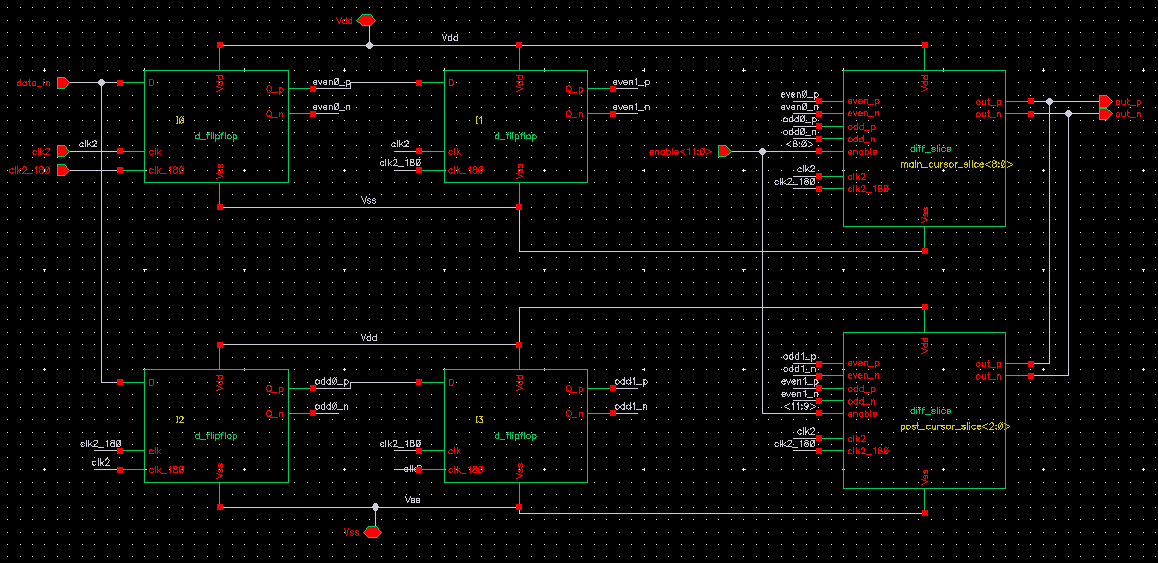
\includegraphics[scale=0.55]{img/transmitter.png}}
  \caption{Transmitter top level circuit}
  \label{fig:top_level}
\end{figure}

\begin{figure}[ht]
  \centering
  \subfigure[Differential slice]
  {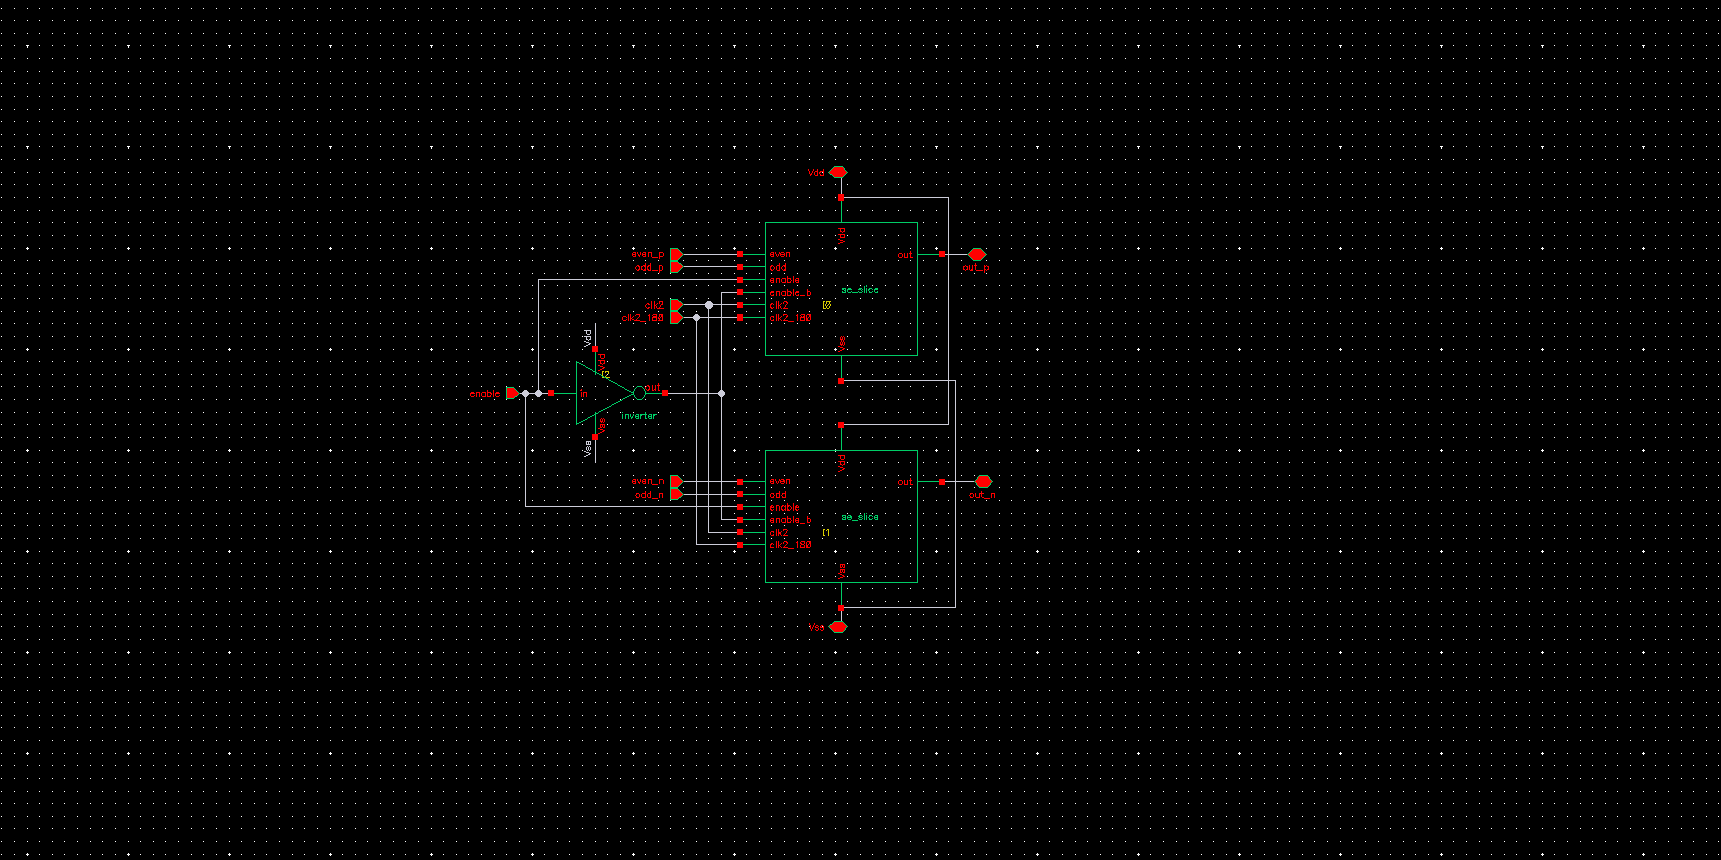
\includegraphics[scale=0.6]{img/diff_slice.png}}
  \subfigure[Single-ended slice]
  {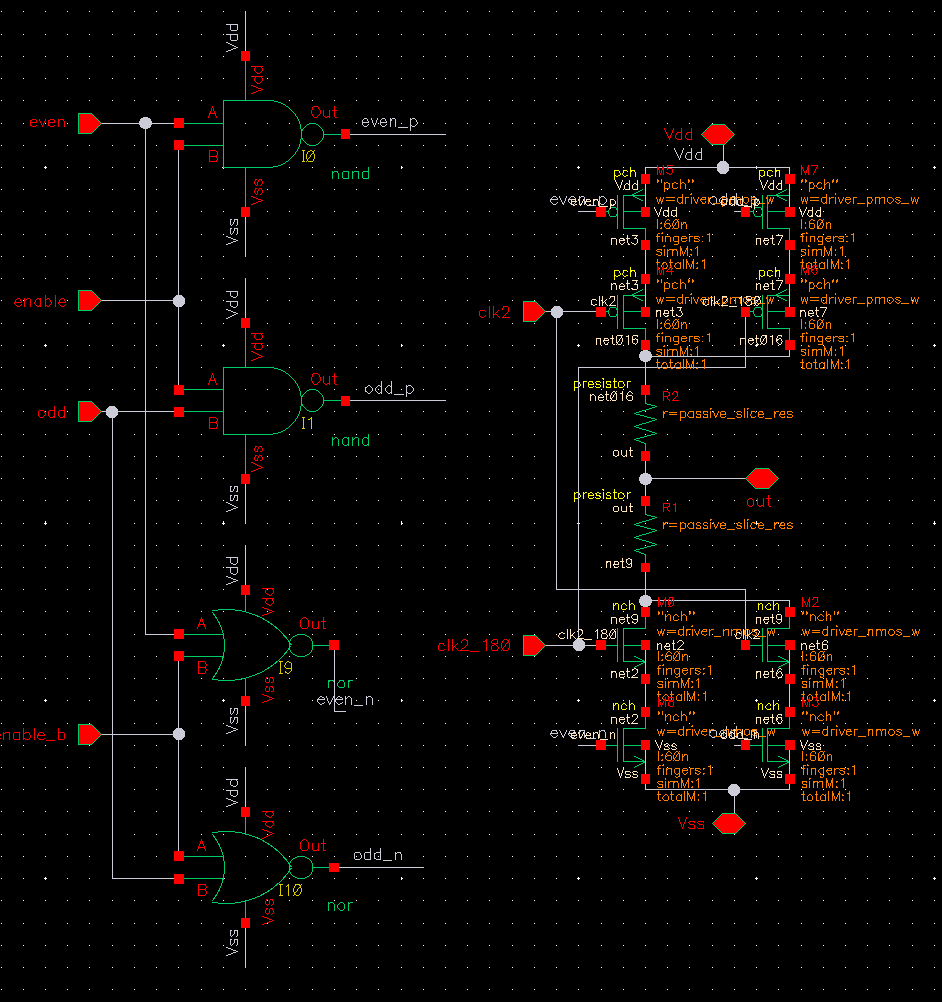
\includegraphics[scale=0.5]{img/se_slice.png}}
  \caption{Slice circuits}
  \label{fig:slices}
\end{figure}

\begin{figure}[ht]
  \centering
  {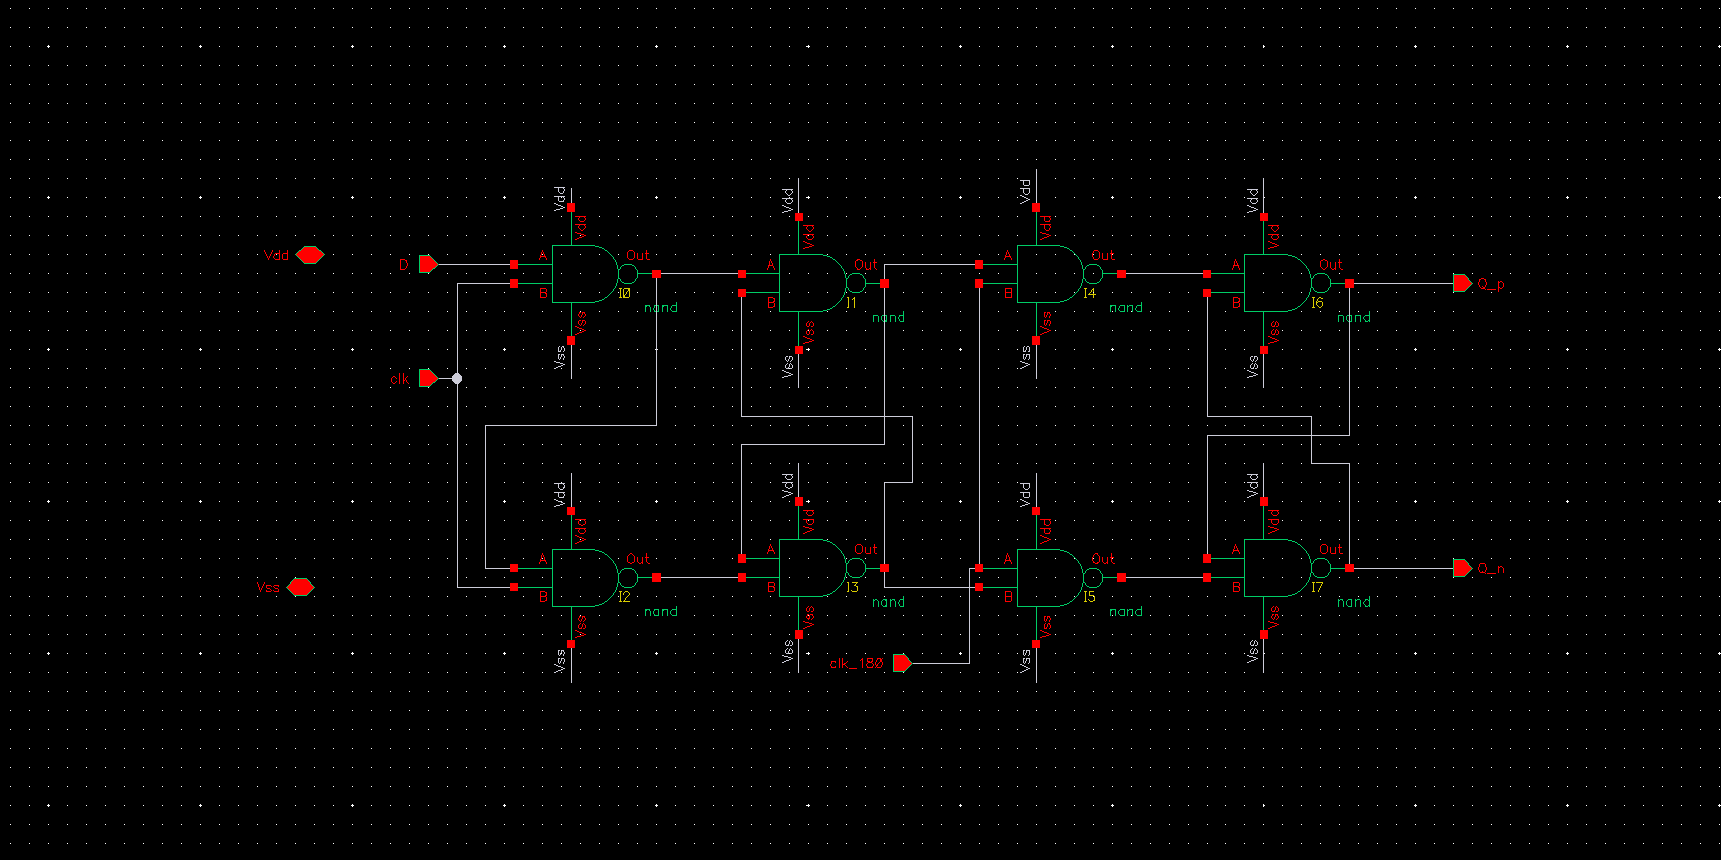
\includegraphics[scale=0.47]{img/flipflop.png}}
  \caption{D-Flipflop}
  \label{fig:flipflop}
\end{figure}

\begin{figure}[ht]
  \centering
  \subfigure[Inverter]
  {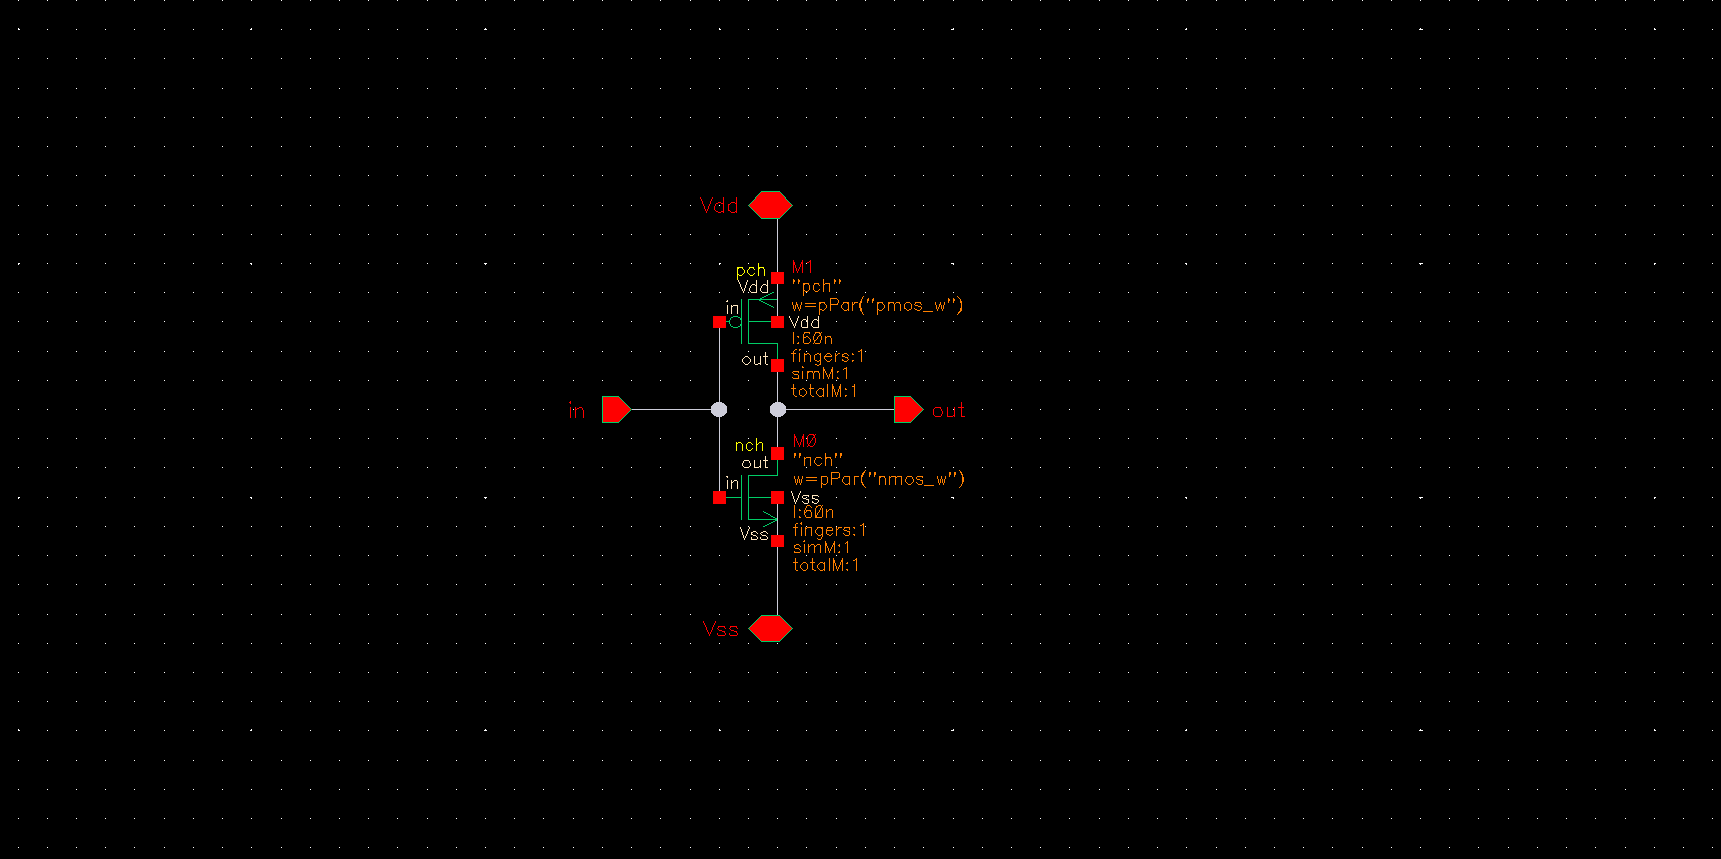
\includegraphics[scale=0.5]{img/inverter.png}}
  \subfigure[NAND gate]
  {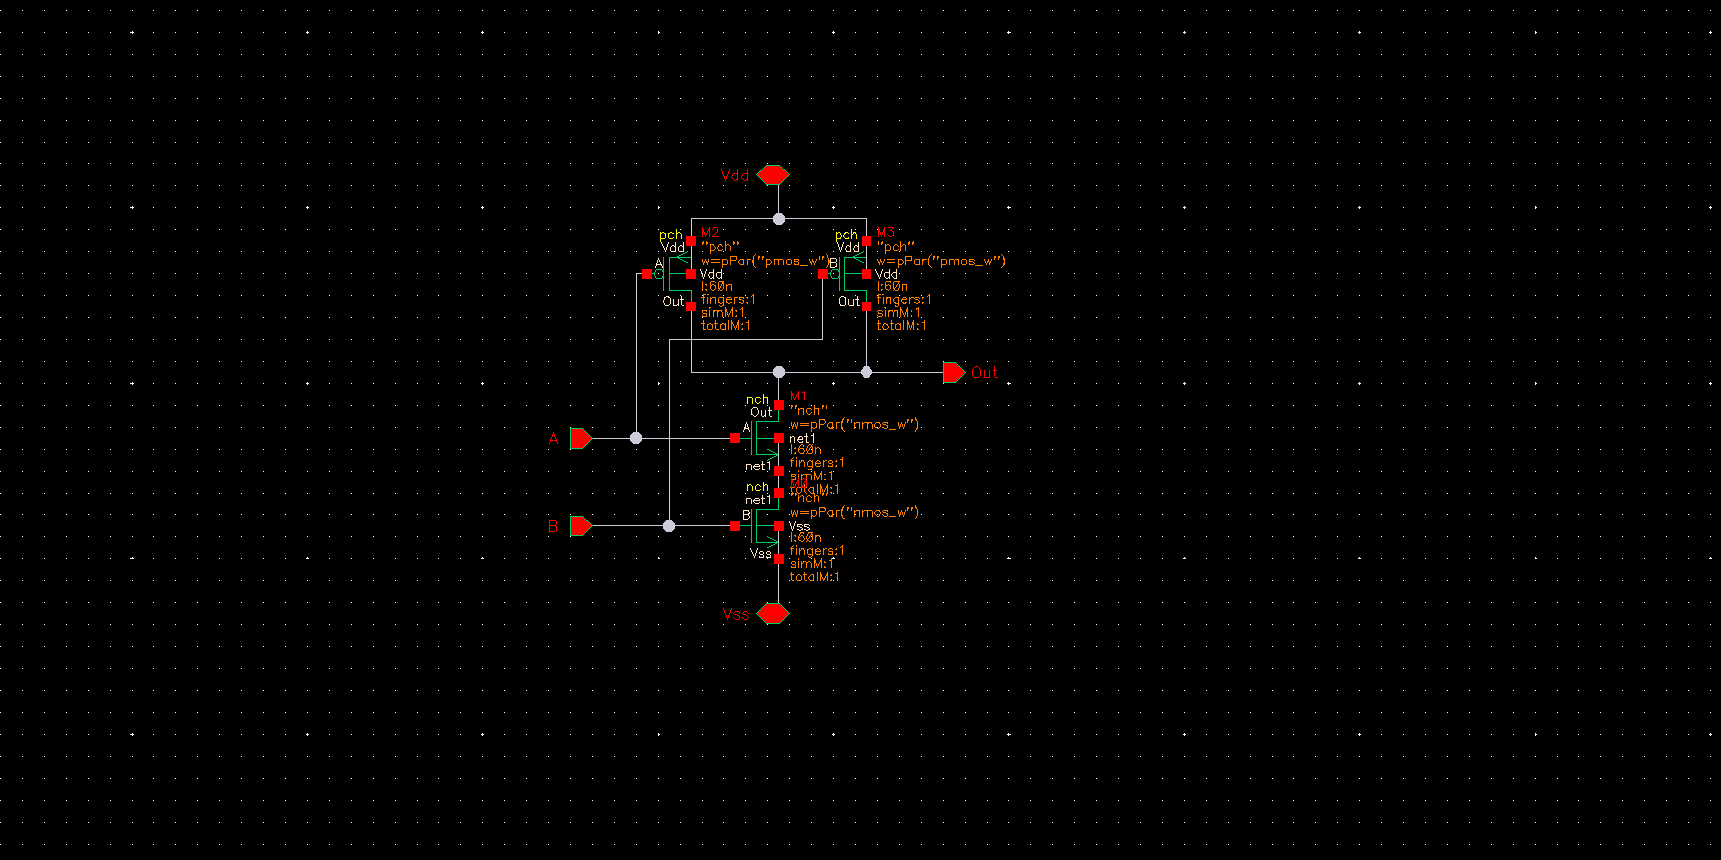
\includegraphics[scale=0.5]{img/nand.png}}
  \subfigure[NOR gate]
  {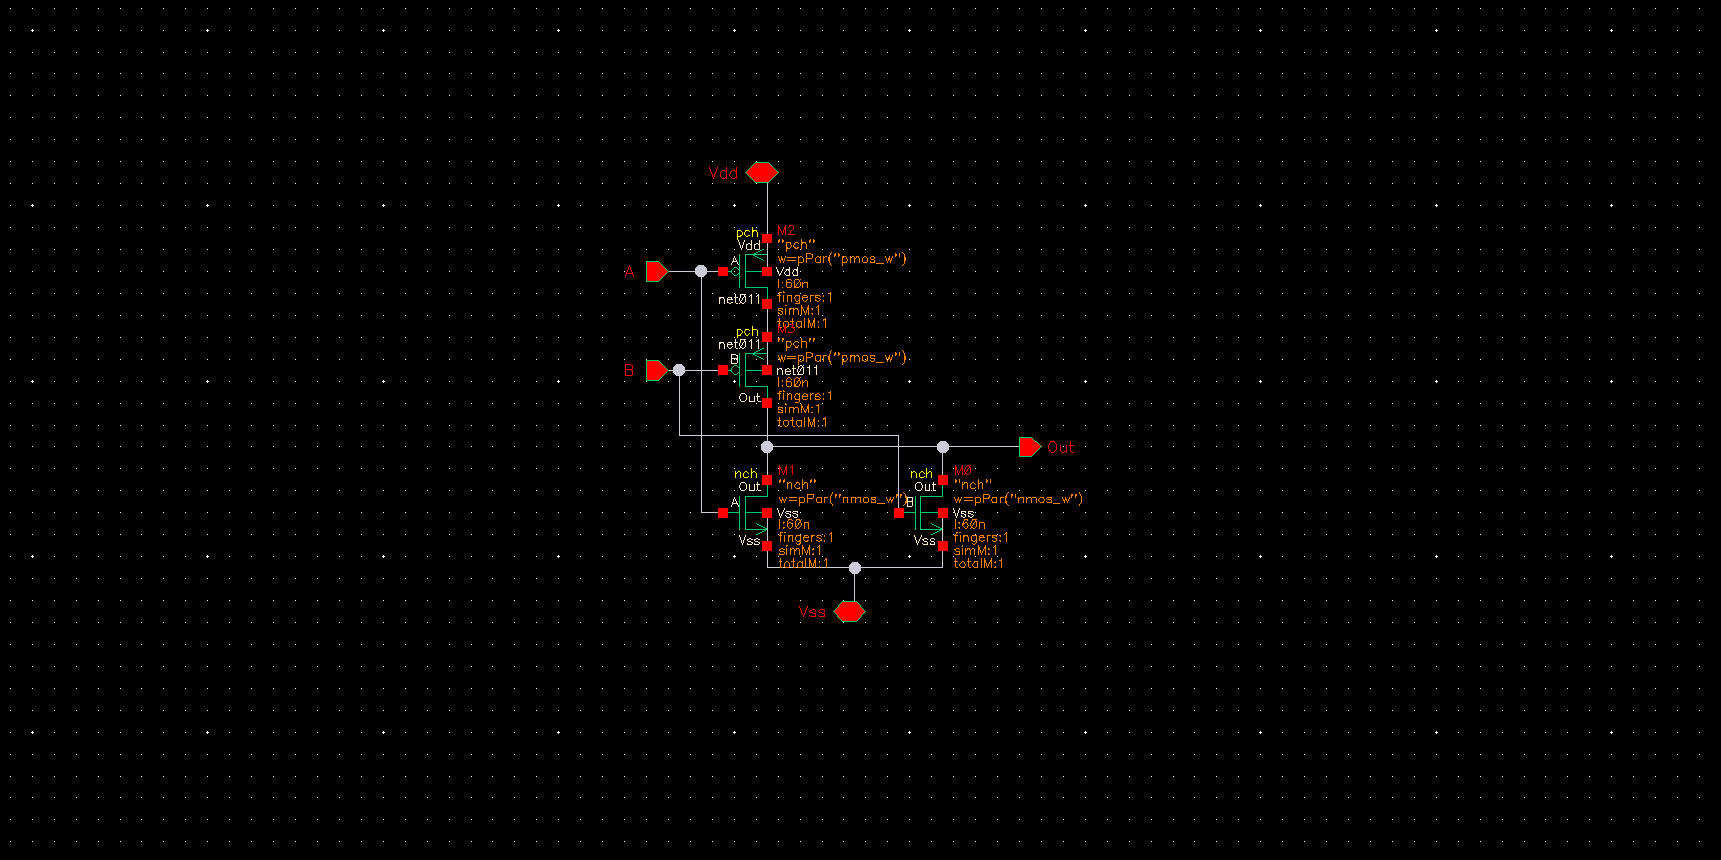
\includegraphics[scale=0.5]{img/nor.png}}
  \caption{Simple gate circuits}
  \label{fig:gates}
\end{figure}